\documentclass[11pt]{article}
\usepackage[margin=0.85in]{geometry}
\usepackage{amsmath,amssymb,bm,booktabs,longtable,array,graphicx,xcolor,enumitem,listings,fancyhdr}
\usepackage[T1]{fontenc}
\usepackage{lmodern,microtype}
\setlength{\emergencystretch}{3em}
\usepackage[colorlinks=true,linkcolor=teal,urlcolor=teal,citecolor=teal]{hyperref}
\definecolor{ink}{HTML}{17334A}
\lstset{basicstyle=\ttfamily\footnotesize,breaklines=true,columns=fullflexible,frame=single,rulecolor=\color{gray},showstringspaces=false}
\setlist{nosep,leftmargin=*}
\setlength{\parindent}{0pt}\setlength{\parskip}{6pt}
\pagestyle{fancy}\fancyhf{}\lhead{PCA: theory and professional practice}\rhead{Khan}\cfoot{\thepage}\setlength{\headheight}{14pt}
\newcommand{\R}{\mathbb R}\newcommand{\tr}{\operatorname{tr}}\newcommand{\Cov}{\operatorname{Cov}}
\title{\color{ink}Principal Component Analysis\\Theory, Computation, and Research Practice}
\author{Md. Ikramul Haq Khan\\University of Nevada, Las Vegas\\Academic study and reproducible practice notes}
\date{October 29, 2026}
\begin{document}\maketitle
\begin{abstract}
PCA chooses orthogonal directions that retain maximal variance, or equivalently give minimal squared reconstruction error, for a specified representation of the data. Professional use requires a scientific objective, justified preprocessing, stable numerical computation, interpretation of scores and loadings, and validation suited to the intended decision. These notes connect linear algebra and probability to real manufacturing and biomedical applications. They include a hand calculation, an executed biomedical example, Python and R workflows, and a curated reading collection. The manufacturing workflow is a proposed analysis of a real public dataset, not a claim about a deployed commercial system.
\end{abstract}
\tableofcontents\newpage
\section{Start with the decision, not the algorithm}
PCA answers: \emph{Which linear directions describe most of the variation in the measurements we chose, after the transformations and scaling we chose?} It does not automatically answer which variables cause an outcome or which directions predict it best.

Choose the goal before deciding how many components to keep:
\begin{center}\begin{tabular}{p{.20\linewidth}p{.35\linewidth}p{.36\linewidth}}\toprule
Goal & Useful output & Evidence needed\\\midrule
Exploration & Score plots and interpretable variable patterns & Sensitivity to scaling, outliers, batches, and sampling\\
Compression & A low-rank reconstruction & Error on representative future observations\\
Prediction & Components entering a supervised model & Entire preprocessing pipeline validated on unseen units\\
Process monitoring & Score distance and residual distance & Alarm rate and detection performance on future process data\\
Scientific inference & A population subspace or association & Explicit sampling assumptions and appropriate uncertainty\\\bottomrule
\end{tabular}\end{center}
The same variance threshold need not suit all five goals. Retaining 95\% of measured variance is a descriptive choice, not a universal scientific standard.

\section{The theoretical foundation, with dimensions}
\subsection{Data, centering, and scaling}
Let $X\in\R^{n\times p}$ contain $n$ observations in rows and $p$ numerical variables in columns. Let $\bar x\in\R^p$ be its column-mean vector. Define
\[
X_c=X-\bm 1_n\bar x^T,\qquad Z=X_cD^{-1},
\]
where $D=I_p$ for covariance PCA and $D=\operatorname{diag}(s_1,\ldots,s_p)$ for correlation PCA, using positive sample standard deviations. All three data matrices have dimension $n\times p$.

With sample-standardized columns,
\[
S_Z=\frac{Z^TZ}{n-1}=R,\qquad \tr(R)=p.
\]
With centered unscaled columns, $S_Z$ is the original sample covariance matrix. PCA depends on the chosen metric: changing units changes covariance PCA. Standardization makes each variable have equal marginal variance, but can also amplify noisy, low-variance measurements. Hence it needs scientific justification.

\subsection{Variance maximization and the Rayleigh quotient}
For a column vector $a\in\R^p$, the score vector is $t=Za\in\R^n$. Its sample variance is
\[
\frac{t^Tt}{n-1}=a^TS_Za.
\]
Without a constraint, replacing $a$ by $100a$ increases the variance by $10{,}000$, so the problem is unbounded. Impose $a^Ta=1$:
\[
\max_{a^Ta=1}a^TS_Za.
\]
The Lagrangian $L=a^TS_Za-\lambda(a^Ta-1)$ gives
\[
2S_Za-2\lambda a=0\quad\Longrightarrow\quad S_Za=\lambda a.
\]
Order eigenvalues $\lambda_1\ge\cdots\ge\lambda_p\ge0$. PC1 uses a unit eigenvector $v_1$ for $\lambda_1$. Subsequent directions maximize the same criterion subject to orthogonality to previous directions. This is precisely the eigenvalue/Rayleigh-quotient connection from linear algebra.

\subsection{Scores, projections, and reconstruction}
Let $V_k=[v_1,\ldots,v_k]\in\R^{p\times k}$ with $V_k^TV_k=I_k$. Then
\[
\underbrace{T_k}_{n\times k}=\underbrace{Z}_{n\times p}\underbrace{V_k}_{p\times k},\qquad
\underbrace{\widehat Z_k}_{n\times p}=T_kV_k^T=ZP_k,
\quad P_k=V_kV_k^T.
\]
$P_k$ is a $p\times p$ orthogonal projector: $P_k^T=P_k$ and $P_k^2=P_k$. Geometrically, each observation is projected onto a $k$-dimensional plane through the centered origin. Returning to original units gives
\[
\widehat X_k=\bm1_n\bar x^T+\widehat Z_kD.
\]
When scaling is used, this minimizes error in standardized units; it need not minimize unweighted error in original measurement units.

\subsection{The SVD is the computational bridge}
The thin singular value decomposition is
\[
Z=U_r\Delta_rV_r^T,
\]
where $r=\operatorname{rank}(Z)$, $U_r\in\R^{n\times r}$, $V_r\in\R^{p\times r}$, and $\Delta_r=\operatorname{diag}(d_1,\ldots,d_r)$. Thus
\[
S_Z=V_r\frac{\Delta_r^2}{n-1}V_r^T,\qquad
\lambda_j=\frac{d_j^2}{n-1},\qquad T_r=U_r\Delta_r.
\]
Use a direct SVD rather than forming and diagonalizing $Z^TZ$ when numerical stability matters. On the nonzero singular spectrum, forming the cross-product squares the condition number. R's \texttt{prcomp} implements SVD; see reference \ref{ref:r}.

\subsection{The reconstruction optimality identity}
Among all matrices $A$ of rank at most $k$, truncated SVD minimizes $\|Z-A\|_F^2$. Consequently,
\[
\|Z-\widehat Z_k\|_F^2=\sum_{j>k}d_j^2
=(n-1)\sum_{j>k}\lambda_j.
\]
The fraction of retained variance is
\[
\mathrm{PVE}_k=\frac{\sum_{j=1}^{k}\lambda_j}{\tr(S_Z)}.
\]
This is why maximum retained variance and minimum squared reconstruction error are equivalent. The identity holds for the fitted data. Future-data error must be evaluated separately.

\subsection{Rank, singularity, and positive definiteness}
Centering gives $\bm1_n^TZ=0$, hence
\[
r\le\min(n-1,p).
\]
If $p\ge n$, the sample covariance cannot be positive definite. Nevertheless, SVD PCA is well defined: it uses the nonzero directions without inverting the covariance. Duplicate variables and exact linear relationships can lower rank further.

\subsection{Probability: identities versus assumptions}
For a population vector $\mathcal X\in\R^p$ with finite second moments, covariance $\Sigma$ and unit eigenvectors $v_j$, define $Y_j=v_j^T(\mathcal X-\mu)$. Then
\[
\operatorname{Var}(Y_j)=\lambda_j,\qquad
\Cov(Y_j,Y_\ell)=0\quad(j\ne\ell).
\]
These are covariance identities. Gaussianity is not needed to compute PCA or prove reconstruction optimality. Joint Gaussianity does make the population components independent. Without it, zero correlation does not imply independence. Classical confidence statements need additional assumptions about sampling, moments, and sometimes distribution; repeated measures and time series require dependence-aware methods.

\section{A complete hand calculation}
Consider two centered variables with covariance
\[
S=\begin{pmatrix}4&3\\3&4\end{pmatrix}.
\]
The characteristic polynomial is
\[
\det(S-\lambda I)=(4-\lambda)^2-9=(\lambda-7)(\lambda-1).
\]
Thus $\lambda_1=7$, $\lambda_2=1$. Normalized eigenvectors are
\[
v_1=\frac{1}{\sqrt2}\begin{pmatrix}1\\1\end{pmatrix},\qquad
v_2=\frac{1}{\sqrt2}\begin{pmatrix}1\\-1\end{pmatrix}.
\]
PC1 is $Y_1=(X_1+X_2)/\sqrt2$; PC2 is $Y_2=(X_1-X_2)/\sqrt2$. Their variances are $7$ and $1$, while their covariance is zero. The first direction describes shared movement and retains $7/8=87.5\%$ of variance.

For the centered observation $x=(2,0)^T$, $t_1=v_1^Tx=\sqrt2$. Its one-component approximation is $\hat x=t_1v_1=(1,1)^T$. The residual is $(1,-1)^T$, which is perpendicular to $v_1$, and its squared length is $2$. PCA therefore loses the part of this observation lying along the discarded direction.

\begin{figure}[ht]\centering
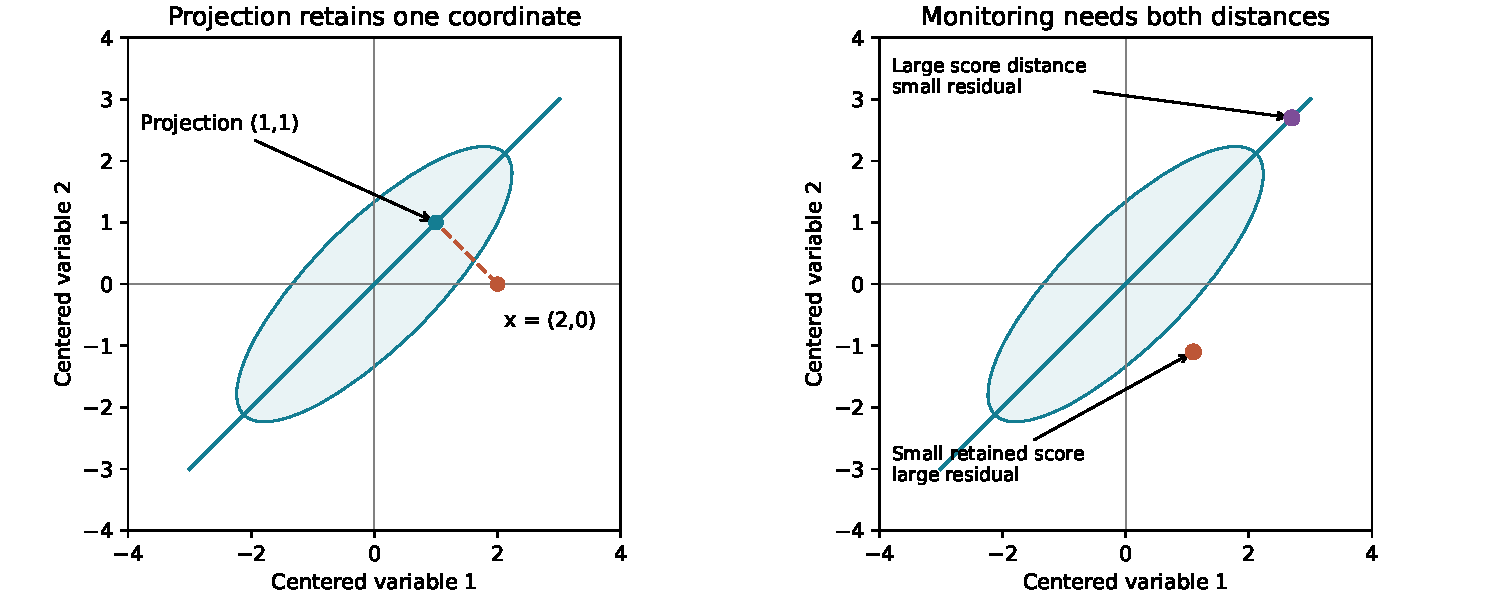
\includegraphics[width=\linewidth]{pca_geometry.pdf}
\caption{Geometric illustration, not observed manufacturing data. Left: a point is projected onto PC1, leaving a perpendicular residual. Right: a point may be extreme within the retained direction or deviate outside it; these motivate the two monitoring statistics in Section 7.}
\end{figure}
\section{Preprocessing that survives professional review}
\begin{enumerate}
\item \textbf{Define an observation.} Patient, visit, specimen, wafer, or batch? A row is not automatically an independent experimental unit.
\item \textbf{Audit variables.} Remove identifiers, outcome labels, timestamps used only as metadata, impossible values, duplicated columns, and constants from the PCA feature matrix. Retain relevant metadata for interpretation.
\item \textbf{Investigate missingness.} Median imputation is a baseline, not a principled answer to every missing-data mechanism. It can suppress variation and alter correlation. Compare suitable alternatives and keep every learned imputation inside training folds.
\item \textbf{Choose transformations.} Skewed positive concentrations may merit logs; RNA-seq needs count-aware normalization and transformation. Do not apply arbitrary logs to signed returns or zero values without a defined measurement model.
\item \textbf{Choose scaling.} Standardize mixed units when equal marginal weighting is defensible. Preserve physical scales when absolute variation is the scientific target. Inspect sensitivity to both when reasonable.
\item \textbf{Choose validation units before fitting.} Split by patient, batch, site, or time according to future use. Estimate imputation, means, scales, and PCA directions from training observations only.
\end{enumerate}
PCA is unsupervised, but fitting it using held-out covariates can still leak information into a predictive evaluation. Pipelines should refit preprocessing in every cross-validation training fold; official guidance is in reference \ref{ref:leakage}.

\section{How many components should be retained?}
\begin{center}\begin{tabular}{p{.23\linewidth}p{.36\linewidth}p{.32\linewidth}}\toprule
Criterion & Appropriate interpretation & Main limitation\\\midrule
Cumulative PVE & Fraction of measured variation retained & Not predictive accuracy or scientific truth\\
Scree elbow & Descriptive change in eigenvalue decay & Can be ambiguous\\
Parallel analysis & Compare observed eigenvalues with a justified null reference & Null simulation must reflect relevant design/dependence\\
External reconstruction & Assess fidelity on new observations & Unpenalized error often improves as $k$ grows\\
Predictive CV & Tune $k$ for a prespecified outcome metric & Needs nesting or a separate final test set\\
Monitoring validation & Balance alarms, missed faults, and delay & Large-variance directions can miss subtle faults\\\bottomrule
\end{tabular}\end{center}
The correlation-PCA rule ``retain eigenvalues above 1'' compares to the average eigenvalue. It is a heuristic, not a general test. For reconstruction, include a complexity, storage, or denoising objective: choosing the lowest reconstruction error alone can simply retain every direction.

\section{Interpretation: what loadings actually mean}
A \emph{score} is the coordinate of an observation; an eigenvector coefficient describes a direction in variable space. Software uses ``loading'' for different objects, so state the convention explicitly.

For sample-standardized variables, the correlation loading is
\[
\operatorname{Corr}(Z_\ell,T_j)=\sqrt{\lambda_j}\,v_{\ell j}.
\]
For a general centered variable with sample variance $s_{Z_\ell}^2$, divide this expression by $s_{Z_\ell}$. Squared eigenvector coefficients sum to one within each component; squared correlation loadings generally do not.

\textbf{Signs are arbitrary.} Replacing $v_j$ and $T_j$ by their negatives leaves reconstruction and variance unchanged. Interpret relative signs within a component, not a supposedly intrinsic positive direction.

\textbf{A component is not a discovered biological mechanism.} Label it cautiously using several high-magnitude variables and domain knowledge. Correlated technical factors can dominate the same direction. A biplot also depends on its scaling convention; angles and distances have specific, sometimes approximate interpretations and cannot all be read interchangeably.

\section{Real industry example: semiconductor process monitoring}
\subsection{Dataset and business question}
The public UCI SECOM dataset contains 1,567 production observations and 591 measured features, with missing values, pass/fail labels, and timestamps. UCI reports 104 failures. Its original task concerns manufacturing yield and useful process signals; see reference \ref{ref:secom}. These are real manufacturing data. The PCA workflow below is a proposed training exercise, not a reproduced commercial deployment.

Two different questions are possible: (i) is the process behaving unusually compared with a verified normal baseline? (ii) can measurements predict failure? Monitoring and supervised failure prediction require different validation and should not be conflated.

\subsection{A monitoring workflow}
Select a historically justified, stable normal-operation period. Do not assume that every passing item came from an in-control process. Remove unavailable/constant channels using the baseline, handle missingness with engineering review, and fit the baseline scaler and PCA. Reserve a separate baseline calibration period and then future observations for evaluation. Fit separate models for genuinely different operating modes when justified.

For a new standardized measurement $z\in\R^p$, compute
\[
t=V_k^Tz,\quad \hat z=V_kt,\quad e=z-\hat z,
\]
\[
T^2(z)=\sum_{j=1}^{k}\frac{t_j^2}{\lambda_j},\qquad Q(z)=e^Te.
\]
Here $T^2$ is squared Mahalanobis distance within the retained subspace, requiring positive retained eigenvalues. $Q$, also called squared prediction error, measures departure from that subspace. NIST discusses PCA control charts and the value of accompanying variable-level charts in reference \ref{ref:nist}.

\begin{center}\begin{tabular}{p{.22\linewidth}p{.65\linewidth}}\toprule
Pattern & Interpretation to investigate\\\midrule
Large $T^2$, modest $Q$ & An extreme combination along familiar process relationships\\
Modest $T^2$, large $Q$ & A broken relationship or new pattern outside the fitted plane\\
Both large & A substantial departure in both location and structure\\\bottomrule
\end{tabular}\end{center}
For example, temperature and pressure may normally move together. A coordinated extreme shift can elevate $T^2$; an unusual disagreement can elevate $Q$. This is an illustrative physical interpretation, not an identified SECOM sensor result: anonymized feature names limit causal diagnosis.

\subsection{Alarm calibration and deployment}
Estimate thresholds on independent normal calibration data, then evaluate the \emph{joint} alarm rule on later data. Two marginal 99th-percentile thresholds do not automatically yield a 1\% overall alarm rate. Serial correlation and repeated monitoring further change operational false-alarm behavior. Classical $F$ or chi-square approximations require their precise assumptions and are not interchangeable between baseline and future monitoring.

Report alarms per production unit, sensitivity to documented faults, detection delay, operating mode, missingness drift, and the consequences of false alarms. Investigate per-variable residuals $e_\ell^2$ to localize deviations; these are diagnostic contributions, not proof of root cause. Freeze and version feature order, units, transformations, imputer, scaler, eigenvectors, eigenvalues, $k$, thresholds, and calibration dates.

For \emph{failure prediction}, compare a PCA-plus-classifier pipeline with no-PCA regularized baselines. With only 104 failures, accuracy alone can be misleading; report precision-recall performance, sensitivity at an actionable false-positive rate, and probability calibration. Use chronological or batch-aware evaluation when these match deployment.

\section{Real biomedical research: RNA-seq quality assessment}
\subsection{Why raw-count PCA is usually the wrong starting point}
RNA-seq records counts for genes across biological samples. High counts tend to have different variability from low counts, and library sizes differ. DESeq2 supplies variance-stabilizing and regularized-log transformations for exploration; its vignette demonstrates sample PCA. The transformations serve visualization, while differential-expression estimation uses a count model, not the displayed PC scores; see reference \ref{ref:deseq}.

A suitable workflow is count QC, low-information filtering, size-factor normalization and variance stabilization, then sample PCA annotated by biological condition, donor, batch, and quality metrics. If expression is genes-by-samples, transpose it before \texttt{prcomp} so that observations are samples.

\begin{lstlisting}[language=R]
# Requires a real counts matrix and matching sample metadata.
# counts: genes x samples; coldata: samples x metadata columns.
# colnames(counts) must equal rownames(coldata).
library(DESeq2)
stopifnot(identical(colnames(counts), rownames(coldata)))
dds <- DESeqDataSetFromMatrix(countData=counts,
    colData=coldata, design=~ batch + condition)
dds <- dds[rowSums(counts(dds)) >= 10, ]
# blind=FALSE uses design-aware dispersion information; select this
# deliberately. For unbiased sample QA, also consider blind=TRUE.
vsd <- vst(dds, blind=FALSE)
plotPCA(vsd, intgroup=c("condition", "batch"))
# This plot uses its own gene-selection default; report ntop.
# Explicit alternative: PCA on a stated number of variable genes.
rv <- apply(assay(vsd), 1, var)
keep <- head(order(rv, decreasing=TRUE), min(500, length(rv)))
p <- prcomp(t(assay(vsd)[keep, ]), center=TRUE, scale.=FALSE)
summary(p)
\end{lstlisting}
This code is a template requiring actual counts and metadata; it was not executed for these notes. The filtering and 500-gene choice are examples, not universal thresholds. The fast \texttt{vst} function also requires sufficient eligible genes; use the documented alternative when that condition fails.

\subsection{What the plot can and cannot establish}
If samples separate by treatment, investigate whether treatment is confounded with sequencing batch. If every treated sample is in one batch and every control is in another, PCA cannot identify which caused separation; a batch-adjusted model may itself be unidentifiable. Do not automatically remove PCs or outlying samples merely to improve group separation. Check sample identity, technical quality, protocol deviations, and prespecified exclusions.

A PCA plot is exploratory evidence, not a differential-expression test, a treatment-effect estimate, or a valid post-selection significance test. If variables are selected using outcomes before PCA, that selection must be disclosed and included in predictive validation where relevant.

\section{Executed computational example: breast-cancer measurements}
\subsection{Dataset, split, and verified results}
The scikit-learn Wisconsin Diagnostic Breast Cancer dataset contains 569 observations and 30 numerical features derived from cell-nucleus measurements, with benign/malignant labels; see reference \ref{ref:data}. We use it as an educational benchmark, not as evidence of clinical validity.

The companion Python script uses an 80/20 stratified split with seed 761: 455 training observations and 114 held-out observations. Scaling and exploratory PCA are fitted using training measurements only. With the script's class encoding and split, the executed component summaries appear below; exact output is recorded in \texttt{results.json}.
\begin{center}\begin{tabular}{lrr}\toprule
Component & Variance (\%) & Cumulative (\%)\\\midrule
PC1 & 44.26 & 44.26\\
PC2 & 19.15 & 63.41\\
PC3 & 9.43 & 72.84\\
PC4 & 6.74 & 79.58\\
PC5 & 5.51 & 85.09\\\bottomrule
\end{tabular}\end{center}
Ten components retain at least 95\% of training variance. The first two retain about 63.4\%, so the visible scatterplot omits about 36.6\%. Labels are overlaid after PCA; no labels enter the PCA optimization.
\begin{figure}[ht]\centering
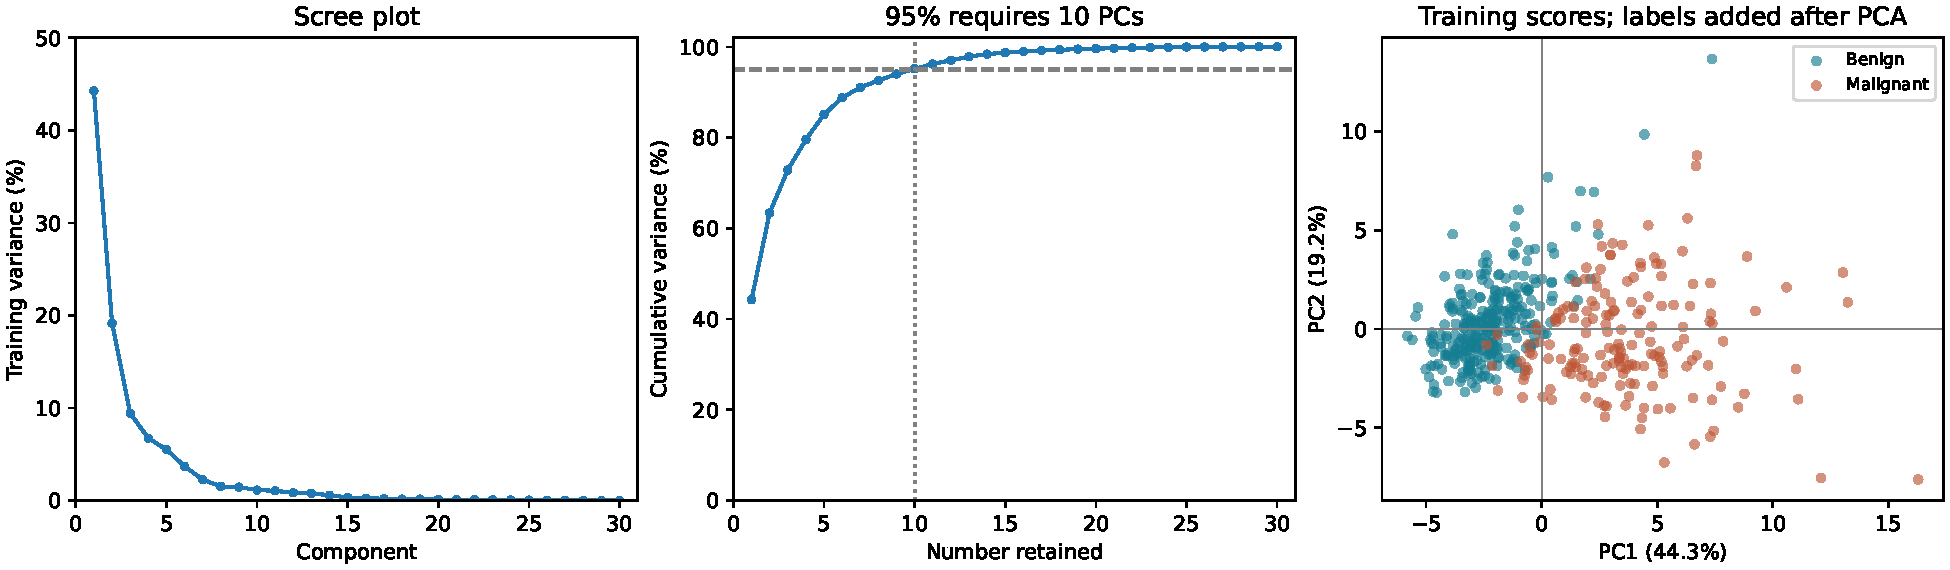
\includegraphics[width=\linewidth]{biomedical_pca.pdf}
\caption{Executed training-data analysis. Left: eigenvalue proportions. Middle: cumulative proportion and the 95\% threshold. Right: PC scores with diagnosis labels added for interpretation. Axes include the origin. Apparent separation does not quantify clinical performance.}
\end{figure}

\subsection{Predictive evaluation without leakage}
The script compares $k\in\{2,5,10,15,20\}$ and a no-PCA representation, jointly with four logistic-regression regularization strengths. Five-fold stratified cross-validation is performed entirely within the 455 training cases; each fold refits its own scaler and PCA. The selected pipeline is evaluated once on the 114-case test set. This is a tuning-plus-holdout design, not nested CV.

In the executed run, cross-validation selected five PCs and logistic regression with $C=1$. Test ROC AUC was 0.9934, average precision 0.9909, and Brier score 0.0247 (malignancy is the positive class). The separate ten-PC representation had standardized test reconstruction MSE 0.0822. These are one-split educational benchmark results with substantial sampling uncertainty, not externally validated clinical estimates.

It reports ROC AUC, average precision, Brier score, and test reconstruction error. The best representation may be no PCA; that is an informative result. A serious clinical study additionally needs uncertainty intervals, threshold-specific sensitivity/specificity, calibration curves, subgroup assessment where justified, and external validation across sites or time. This small educational split is insufficient for deployment.

\subsection{Computational verification}
The executed script checks
\[
V^TV=I,\quad \widehat{\Cov}(T)=\operatorname{diag}(\lambda_j),\quad
\|Z-\widehat Z_k\|_F^2=(n-1)\sum_{j>k}\lambda_j.
\]
\texttt{StandardScaler} uses a population-denominator variance ($n$), whereas sample PCA eigenvalues use $n-1$. Therefore its scaled training matrix has total \emph{sample} variance $pn/(n-1)$, not exactly $p$. Explained-variance proportions remain consistent under this common overall scaling factor. This explains small differences from R's sample-SD standardization.

\section{An R workflow connecting directly to course notation}
The following self-contained example uses the built-in real USArrests dataset for computational practice. Its observational state-level measurements should not be interpreted as individual-level causal effects. R code is provided for independent practice; the executed results above are from Python.
\begin{lstlisting}[language=R]
X <- as.matrix(USArrests)
p <- prcomp(X, center=TRUE, scale.=TRUE)
V <- p$rotation                  # p x p eigenvector coefficients
T <- p$x                         # n x p observation scores
lambda <- p$sdev^2
pve <- lambda / sum(lambda)
k <- which(cumsum(pve) >= 0.90)[1]
Z <- scale(X, center=p$center, scale=p$scale)
Zhat <- T[,1:k,drop=FALSE] %*% t(V[,1:k,drop=FALSE])
stopifnot(max(abs(crossprod(V)-diag(ncol(X)))) < 1e-8)
stopifnot(max(abs(cov(T)-diag(lambda))) < 1e-8)
stopifnot(abs(sum((Z-Zhat)^2) -
    (nrow(X)-1)*sum(lambda[-seq_len(k)])) < 1e-7)
# Correlation loadings, not just eigenvector coefficients:
L <- sweep(V, 2, sqrt(lambda), '*')
print(round(L, 3))
# New observations: reuse the fitted means, SDs, and directions.
new_scores <- predict(p, newdata=X[1:2,,drop=FALSE])
# Above rows merely illustrate the API, not independent validation.
\end{lstlisting}
In an actual prediction task, fit \texttt{prcomp} only on the training fold, then call \texttt{predict} on validation observations. Avoid fitting a full-data PCA first and cross-validating only the regression.

\section{Advanced practice: stability, high dimension, and alternatives}
\subsection{Eigenvalue gaps and subspace uncertainty}
When two population eigenvalues are equal, individual eigenvectors in their eigenspace are not uniquely defined. Nearly equal sample eigenvalues often produce unstable individual directions. The combined subspace can still be stable. Thus sign-aligning bootstrap eigenvectors is necessary but sometimes insufficient: allow rotations within nearly tied blocks.

For two orthonormal loading bases $V_k$ and $W_k$, singular values of $V_k^TW_k$ equal $\cos\theta_j$, where $\theta_j$ are principal angles. Another useful comparison is
\[
\|V_kV_k^T-W_kW_k^T\|_F.
\]
These compare subspaces without mistaking a sign flip or basis rotation for a scientific change. Bootstrap at the true sampling unit: resample patients, batches, or time blocks as appropriate. Refit preprocessing in each resample and compare directions in a consistent coordinate system. State whether $k$ is fixed or reselected.

\subsection{High-dimensional PCA}
Having a computable SVD does not guarantee reliable population directions. When $p$ is large relative to $n$, noisy sample eigenvalues can look substantial and sample eigenvectors can be inaccurate. The behavior depends on signal strength, dimensional growth, and covariance structure, not a universal observations-per-variable rule. Johnstone and Paul provide an advanced orientation in reference \ref{ref:highdim}.

\subsection{Probabilistic PCA and factor analysis}
Probabilistic PCA introduces the model
\[
x=\mu+Wh+\epsilon,\qquad h\sim N_k(0,I_k),\quad
\epsilon\sim N_p(0,\sigma^2I_p),\quad h\perp\epsilon,
\]
where $W\in\R^{p\times k}$. Therefore $\Cov(x)=WW^T+\sigma^2I_p$. Isotropic residual variance is a modeling assumption. Factor analysis typically permits variable-specific residual variances through a diagonal matrix $\Psi$. This distinguishes a distributional latent-variable model from ordinary PCA's geometric optimization. See Tipping and Bishop, reference \ref{ref:ppca}.

\begin{center}\begin{tabular}{p{.24\linewidth}p{.33\linewidth}p{.34\linewidth}}\toprule
Situation & Consider & What must be checked\\\midrule
A few anomalous rows & Robust covariance/subspace estimation & Outlier mechanism and robust tuning\\
Sparse cell corruption & Low-rank plus sparse decomposition & Identifiability; different from all robust PCA methods\\
Interpretability & Sparse PCA & Penalty tuning; orthogonality properties vary\\
Curved structure & Kernel PCA or other nonlinear methods & Out-of-sample behavior and interpretation\\
Very large matrices & Randomized or incremental SVD & Approximation error, convergence, reproducibility\\
Trajectories over time & Functional PCA & Smoothing, alignment, observation density\\
Outcome-focused reduction & PLS or supervised methods & Leakage and outcome-specific validation\\\bottomrule
\end{tabular}\end{center}
PCA on a discretized epidemic curve is possible, but it is not automatically the best way to study total infection burden. If burden is your target, define the integral and uncertainty first; use curve components only if shape variation answers an additional scientific question. Equalizing each time point's variance changes which curve differences receive weight.

\section{A review-ready analysis checklist}
Before interpreting or publishing results, document:
\begin{enumerate}
\item Scientific question, sampling unit, population, inclusion criteria, $n$, $p$, feature definitions, units, and provenance.
\item Missingness by variable and group, transformations, scaling, constant-feature rules, and rationale.
\item Covariance versus correlation PCA, centering, algorithm, numerical tolerances, seed where needed, and software versions.
\item Rank, eigenvalue spectrum, retained $k$, selection criterion, and all data used for selection.
\item Scree and cumulative plots; scores labeled with variance percentages; coefficient or correlation-loading plots with explicit conventions.
\item Outlier and batch investigations; sensitivity to preprocessing; resampling stability where scientific claims depend on components.
\item Task-specific validation: external reconstruction, prediction, or process-monitoring performance. Include a no-PCA comparator for prediction.
\item Limitations: missing dimensions, uncertain directions, sample representativeness, dependence, confounding, and lack of causal identification.
\item Reproducible code, environment, feature order, trained transformation, and a traceable model version if used operationally.
\end{enumerate}
Do not delete valid observations just because they are distant in a PCA plot. An unusual patient may be scientifically important. Distinguish a measurement error, a valid rare observation, and an observation poorly represented by the retained subspace.

\section{Cumulative practice with answers}
\textbf{1.} A centered matrix has 40 rows and 100 columns. Can its covariance be invertible?\\
\emph{Answer:} No. Its rank is at most 39. There can be at most 39 positive sample eigenvalues. SVD PCA is still feasible.

\textbf{2.} PC1 and PC2 explain 80\% of predictor variance. Does a regression using them retain 80\% of predictive information?\\
\emph{Answer:} No. PVE measures predictor variation. An outcome could depend primarily on a discarded direction.

\textbf{3.} A software update reverses PC1 and every PC1 score. Has the fitted subspace changed?\\
\emph{Answer:} No. Both $tv^T$ and $vv^T$ are unchanged when both signs reverse.

\textbf{4.} A process observation has small $T^2$ but large $Q$. Is it necessarily safe?\\
\emph{Answer:} No. Its retained scores are ordinary, but its residual pattern is unusual; a familiar sensor relationship may have broken.

\textbf{5.} Why can test error be optimistic if only scaling, not outcomes, used the test set?\\
\emph{Answer:} The learned representation already incorporated the evaluation observations. It no longer measures a pipeline trained solely on the designated training sample.

\textbf{6.} For covariance eigenvalues $(6,3,1)$ and $n=21$, what is the fitted rank-two residual sum of squares?\\
\emph{Answer:} $(n-1)\lambda_3=20$. Retained variance is $9/10=90\%$.

\section{Curated resources for long-term understanding}
The website companion lists these links individually. Read for the question each source answers rather than collecting links without a purpose.
\begin{enumerate}[label={[\arabic*]}]
\item\label{ref:review} Jolliffe and Cadima (2016), \emph{Principal component analysis: a review and recent developments}. Accessible conceptual and mathematical synthesis. \url{https://doi.org/10.1098/rsta.2015.0202}
\item Nature Reviews Methods Primers (2022), \emph{Principal component analysis}. Broad research-methods orientation. \url{https://www.nature.com/articles/s43586-022-00184-w}
\item\label{ref:r} R official \texttt{prcomp} documentation: SVD, scaling, prediction, and output conventions. \url{https://stat.ethz.ch/R-manual/R-devel/library/stats/html/prcomp.html}
\item\label{ref:sklearn} scikit-learn PCA documentation: solver behavior, components, reconstruction and whitening. \url{https://scikit-learn.org/stable/modules/generated/sklearn.decomposition.PCA.html}
\item\label{ref:leakage} scikit-learn common pitfalls: leakage and training-only preprocessing. \url{https://scikit-learn.org/stable/common_pitfalls.html}
\item\label{ref:nist} NIST/SEMATECH, principal components control charts: industrial monitoring and limitations of multivariate alarms. \url{https://itl.nist.gov/div898/handbook/pmc/section3/pmc342.htm}
\item\label{ref:secom} McCann and Johnston (2008), UCI SECOM dataset. Real semiconductor measurements, missingness, yield labels, and provenance. \url{https://archive.ics.uci.edu/dataset/179/secom}
\item\label{ref:deseq} Love, Anders and Huber, DESeq2 vignette: transformed counts, sample PCA, and separation from differential-expression inference. \url{https://bioconductor.org/packages/release/bioc/vignettes/DESeq2/inst/doc/DESeq2.html}
\item\label{ref:data} scikit-learn Wisconsin Diagnostic Breast Cancer data documentation and source references. \url{https://scikit-learn.org/stable/modules/generated/sklearn.datasets.load_breast_cancer.html}
\item Patterson, Price and Reich (2006), \emph{Population Structure and Eigenanalysis}. Primary research connecting PCA, genetic structure and significance theory. \url{https://doi.org/10.1371/journal.pgen.0020190}
\item\label{ref:ppca} Tipping and Bishop (1999), \emph{Probabilistic Principal Component Analysis}. A likelihood-based latent-variable interpretation. \url{https://www.microsoft.com/en-us/research/wp-content/uploads/2016/02/bishop-ppca-jrss.pdf}
\item\label{ref:highdim} Johnstone and Paul (2018), \emph{PCA in High Dimensions: An Orientation}. Signal, noise, eigenvector inconsistency, and random-matrix ideas. \url{https://pmc.ncbi.nlm.nih.gov/articles/PMC6167023/}
\item Zou, Hastie and Tibshirani (2006), \emph{Sparse Principal Component Analysis}. Sparse directions and interpretability tradeoffs. \url{https://web.stanford.edu/~hastie/Papers/spc_jcgs.pdf}
\item Candes and collaborators, \emph{Robust Principal Component Analysis?} Low-rank plus sparse matrix recovery; inspect the model assumptions. \url{https://statistics.stanford.edu/technical-reports/robust-principal-component-analysis}
\item Halko, Martinsson and Tropp (2011), \emph{Finding Structure with Randomness}. Large-scale approximate decompositions. \url{https://tropp.caltech.edu/papers/HMT11-Finding-Structure.pdf}
\end{enumerate}
\textbf{A sustainable reading sequence.} First use Sections 2--3 to connect eigenvalues, covariance, and projections (about 45--60 minutes). Then run the biomedical script and inspect its three plots (about 45 minutes). Next compare the manufacturing and RNA-seq objectives (about 30 minutes). Study high-dimensional and probabilistic extensions afterward as needed; each primary paper deserves its own reading session.

\appendix\section{Complete reproducible Python implementation}
Run \texttt{python pca\_biomedical.py} in a folder where outputs may be written. Dependencies are NumPy, pandas, Matplotlib and scikit-learn. The downloadable source bundle includes figures, results, environment versions, this script, and this LaTeX source. The analysis uses packaged public data; no patient-identifiable information is collected.
\lstinputlisting[language=Python]{pca_biomedical.py}
\end{document}
